\documentclass{beamer}
 \usetheme{Dresden}
\usecolortheme{whale}

\title{Discrete Random Variable}
\author{Aditya Raj}
\institute{GKCIET, Malda \\ Department of Computer Science and Engineering  \\ Roll No: 35530824051}
\date{February, 2025}

\begin{document}

\begin{frame}
    \titlepage
\end{frame}

\begin{frame}
    \tableofcontents
\end{frame}

\section{Introduction}
\subsection{Random Variable}
\subsection{Types of Random Variable}
\begin{frame}
    \frametitle{Introduction}
    \textbf{What is a Random Variable?} \\
    A random variable (or stochastic variable) is a function which assigns a number to each point of a sample space. It is usually denoted by capital letters such as $X$ and $Y$. \\
    Mathematically, \\
    $$X: \Omega \rightarrow \mathbb{R}$$
    The set of values $x$ of random variable $X$ such that $P(X= x) > 0$ is called the 'support' of $X$.

    \textbf{Types of Random Variable}
    \begin{itemize}
        \item Discrete Random Variable - It takes a finite or countably infinite number of values.
        \item Nondiscrete Random Variable - It can take a noncountably infinite number of values.
    \end{itemize}
\end{frame}

\section{Example of Discrete Random Variable}
\begin{frame}
    \frametitle{Example of Discrete Random Variable}
    Consider an experiment where we toss a fair coin twice. The sample space consists of four possible outcomes: $S = \{HH, HT, TH, TT\}$. Here are some random variables on this space:
    \begin{enumerate}
        \item Let $X$ be the number of Heads. Then,
        $$X(HH) = 2, \quad X(HT) = 1, \quad X(TH) = 1, \quad X(TT) = 0$$
        \item Let $Y$ be the number of Tails. In terms of $X$, $Y = 2 - X$. Or
        $$Y(HH) = 0, \quad Y(HT) = 1, \quad Y(TH) = 1, \quad Y(TT) = 2$$
        \item Let $I$ be 1 if the first toss lands Heads and 0 otherwise.
        $$I(HH) = 1, \quad I(HT) = 1, \quad I(TH) = 0, \quad I(TT) = 0$$
    \end{enumerate}

\end{frame}

\begin{frame}
    This is an example of what is called an indicator random variable since it indicates whether the first toss lands Heads, using 1 to mean “yes” and 0 to mean “no”.  
    \\
    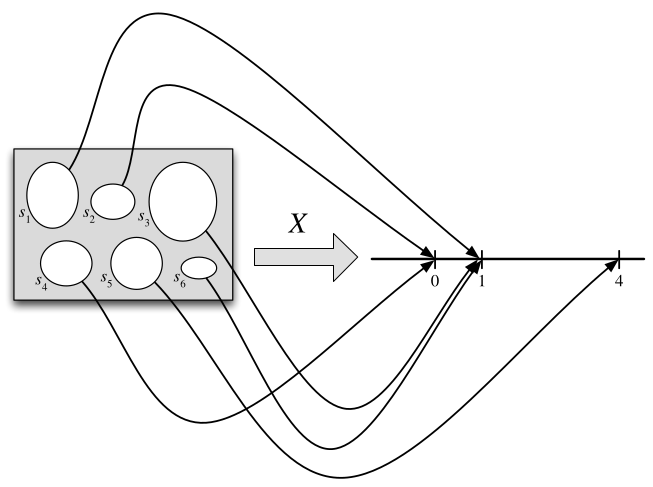
\includegraphics[width=0.5\textwidth]{randomvariable.png}
    \\
    Fig.: A random variable maps the sample space into the real line
\end{frame}
     
\section{Distribution Of Random Variable}
\subsection{Probability Mass Function}
\begin{frame}
    \frametitle{Distribution of Random Variable}
    The distribution of a random variable specifies the probabilities of all events associated with that random variable. For discrete random variables, we generally use the probability mass function (PMF).

    The probability mass function (PMF) of a discrete random variable $X$ is the function $p_X$ given by:
    $$p_X (x) = P (X = x)$$
    Note that this is positive if $x$ is in the support of $X$, and $0$ otherwise.

    Here, $X = x$ denotes an event, consisting of all outcomes $s$ to which $X$ assigns the number $x$. Formally,
    $${X = x} \equiv {s \in S : X(s) = x}$$
\end{frame}

\subsection{Example of PMF}
\begin{frame}
    \frametitle{Example of PMF}
    Using the previous example of two coin tosses, let us find PMFs of random variables $X$, $Y$, and $I$.
    \begin{itemize}
        \item For $X$:
        $$p_X (0) = P (X = 0) = \frac{1}{4}, \quad p_X (1) = P (X = 1) = \frac{1}{2},$$ $$ \quad p_X (2) = P (X = 2) = \frac{1}{4}$$
        and $p_X (x) = 0$ for all other values of $x$.
        
        \item For $Y$:
        \[p_Y (0) = P (Y = 0) = \frac{1}{4}, \quad p_Y (1) = P (Y = 1) = \frac{1}{2},\] \[ \quad p_Y (2) = P (Y = 2) = \frac{1}{4}\]
        and $p_Y (y) = 0$ for all other values of $y$.
    \end{itemize} 
\end{frame}


\begin{frame}
    \begin{itemize}
        \item For $I$:
        $$p_I (0) = P (I = 0) = \frac{1}{2}, \quad p_I (1) = P (I = 1) = \frac{1}{2}$$
        and $p_I (i) = 0$ for all other values of $i$.
    \end{itemize}
    
    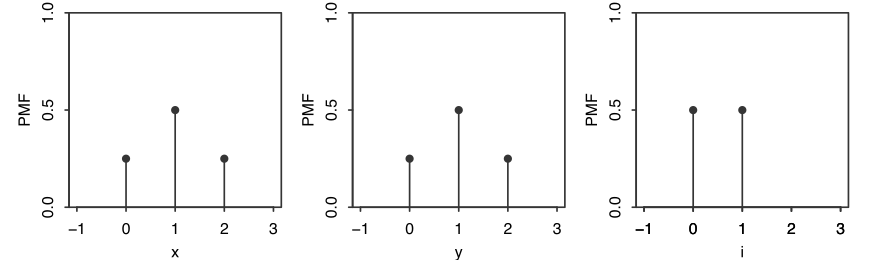
\includegraphics[width=1\textwidth]{pmf.png}
    
    Fig.: Pictorial representation of PMF for random variables $X$, $Y$ and $I$
    % Link for inserted image can be added here

\end{frame}
        
\subsection{Valid PMFs}
\begin{frame}
    \frametitle{Valid PMFs}
    Let $X$ be a discrete random variable with support $x_1, x_2, \ldots$. The PMF $p_X$ of $X$ must satisfy the following two criteria:
    \begin{enumerate}
        \item Nonnegative: $p_X (x) > 0$ if $x = x_j$ for some $j$, and $p_X (x) = 0$ otherwise.
        \item Sums to 1: 
        $$\sum_{j=1}^{\infty} p_X(x_j) = 1$$
    \end{enumerate}
\end{frame}

\subsection{Binomial Distribution}
\begin{frame}
    \frametitle{Binomial Distribution}
\end{frame}
\section{References}
\begin{frame}
    \frametitle{References}
    \begin{enumerate}
        \item Blitzstein, Joseph K., and  Hwang, Jessica. \textit{Introduction to Probability}. 2nd ed., Chapman and Hall/CRC, 2019.
        \item Walrand, Jean. \textit{Probability in Electrical Engineering and Computer Science: An Application-Driven Course}. Springer, 2021.
    \end{enumerate}
\end{frame}

\end{document}